\section{Free selective functors}\label{sec-free}

Free construction with examples

The methodology of building effectful computations with free constructions such
as free~\cite{swierstra2008data} and freer~\cite{kiselyov2015freer} monads and free
applicatives~\cite{free-applicatives} is a widespread in the functional programming community.
It allows to focus on the internal aspects of the effect under consideration and receive the
desired \hs{Applicative} of \hs{Monadic} structure of the computation~\emph{for free},
i.e. without the need to construct instances or prove laws.

In the ``free structures'' methodology, the essence of an effect is a datatype which encodes
the ``commands'' which the effect provides, acting as a deep embedding of the effect's
interface. This datatype must only have enough structure to be a~\hs{Functor}. The purpose of
the free constructions is then to build on top of this functor a richer structure,
which would have the instances of \hs{Applicative}/\hs{Selective}/\hs{Monad}.

\subsection{Free construction}\label{sec-free-construction}

...

\subsection{Ping-pong, freely}\label{sec-free-ping-pong}

To illustrate the usage of the free selective constructor on a simple example, we implement the
Teletype DSL~\cite{swierstra2008data} comprising two commands: reading a string of characters
form the input stream and writing a string to the output stream. The \hs{Teletype} datatype
has two constructors, representing the commands of the Teletype interface:

\begin{minted}[xleftmargin=10pt]{haskell}
data Teletype a = GetLine (String -> a)
                | PutStrLn String a
    deriving Functor
\end{minted}

We embed these commands into the free selective construction with the following two combinators,
mimicking Haskell Prelude's \hs{IO} API:

\begin{minted}[xleftmargin=10pt]{haskell}
getLine :: Select Teletype String
getLine = liftSelect (GetLine id)

putStrLn:: String -> Select Teletype ()
putStrLn s = liftSelect (PutStrLn s ())
\end{minted}

We now can reimplement the \hs{pingPongS} example from the section \ref{sec-intro}
in terms of the free selective construction simply by adjusting the type signature:

\begin{minted}[xleftmargin=10pt]{haskell}
pingPongS :: Select Teletype ()
pingPongS = whenS (fmap (=="ping") getLine) (putStrLn "pong")
\end{minted}

Once we have embedded the \hs{pingPongS} program into the \hs{Select} datatype,
we got access to the machinery for static analysis of effects:

\begin{minted}[xleftmargin=10pt]{haskell}
@\ghci@ getEffects pingPong
[GetLine,PutStrLn pong]
\end{minted}

The \hs{getEffects} function of type \hs{Functor f => Select f a -> [f ()]}
returns a list of all effects of a free selective computation. In the specific case of
the \hs{Teletype} functor, we get a list of all commands that a computation has called.
Internally, the \hs{getEffects} function interprets a free selective computation
in the \hs{Over} functor (see section~\ref{sec-instances}) to construct an over-approximated
list of effects.

We can interpret Teletype programs in any other \hs{Selective} by means of the
\hs{runSelect} function. We must providing a \emph{natural transformation}
\hs{forall a. f a -> g a}, which assigns an interpretation to the commands of
\hs{f} (in our example, \hs{f}~\hs{=}~\hs{Teletype}) in terms of \hs{g}.
A natural example of such a transformation would be an interpretation in the \hs{IO} monad,
which allows to run our \hs{pingPongS} program and get the same behaviour that the
one in \ref{sec-intro} had.

\begin{minted}[xleftmargin=10pt]{haskell}
inIO :: Teletype a -> IO a
inIO (GetLine t)    = t <$> Prelude.getLine
inIO (PutStrLn s x) = Prelude.putStrLn s *> pure x
\end{minted}

\subsection{Build systems, freely}\label{sec-free-build}

...

\subsection{Analysis and simulation of processor instructions}\label{sec-free-isa}

To apply free selective functors to a larger example, we demonstrate
how they can be used for describing the semantics of a hypothetical
instruction set architecture (ISA). The features of the free selective construction will
allow for static data-flow analysis of the instruction semantics, and the possibility
to interpret free selective expressions in any monad will enable us to build a
sequential simulator for programs.

\subsubsection{\textbf{ISA semantics}}

We will represent the semantics of instructions in terms of the following datatype:

\begin{minted}[xleftmargin=10pt]{haskell}
type ISA a = Select RW a
\end{minted}

Here, \hs{Select} is the free selective functor defined earlier in this section.
We apply the \hs{Select} type constructor to the \hs{RW} datatype, which is the
functor we build our free construction on:

\begin{minted}[xleftmargin=10pt]{haskell}
data RW a = Read  Key             (Value -> a)
          | Write Key (ISA Value) (Value -> a)
    deriving Functor
\end{minted}

The \hs{RW} (pronounced read-write) functor encodes the effect of mutable key-value store
comprising two commands.
First, we need to have an ability to \emph{read} a value associated with a key from the store
and second, given a computation which produces a value, \emph{write} its result into the store.
In this example, we fix the values to be machine words and the keys to be the ISA concepts, such
as registers, memory locations and flags.

This exact structure of the definition is required for accommodating a pattern that
occurs frequently in instruction semantics: often we read a value from a register or a memory
cell, do something with the value and then write it somewhere else.
If we had the type of \hs{Write} to be \hs{k -> v -> (v -> a)}, i.e. required
the second argument to be a pure value,
we would not be able to grasp the desired pattern without resorting to the monadic interface.
Additionally, we want the \hs{Write}
operation to not just write the value and return \hs{()}, but to give the just written value
back, so it may be used in the rest of the computations; such a generosity of the \hs{Write}
command not consuming its arguments will be useful to avoid creating more data dependencies
than necessary.

We introduce two convenience combinators, which \emph{lift} the data constructors
of the \hs{RW} datatype into the free selective, thus making them directly usable in
the definitions of instruction semantics:

\begin{minted}[xleftmargin=10pt]{haskell}
read :: Key -> ISA Value
read k = liftSelect (Read k id)

write :: Key -> ISA Value -> ISA Value
write k p = p *> liftSelect (Write k p id)
\end{minted}

Whereas the \hs{read} combinator is exactly the lifted \hs{Read} data constructor,
the \hs{write}'s implementation deserves explanation, since it deviates from the trivial
lifting of the \hs{Write} data constructor and \emph{evaluates its second argument},
thus executing its associated effects.

\subsubsection{\textbf{Example 1. Addition}}

To get acquainted with the vocabulary, we start with a simple semantics for
the addition instruction, which will read the summands from a register and a memory cell,
add them, write the result back into the register and also update the state of the \hs{Zero}
and flag to indicate if the sum was zero:

\begin{minted}[xleftmargin=10pt]{haskell}
add :: Register -> Address -> ISA Value
add reg addr = let arg1     = read (Reg reg)
                   arg2     = read (Mem addr)
                   result   = (+)  <$> arg1   <*> arg2
                   isZero   = (==) <$> pure 0 <*> write (Reg reg) result
               in write (F Zero)     (fromBool <$> isZero)
\end{minted}

Here, we get two effectful values from the two locations and calculate three intermediate
results. To calculate the sum we just lift \hs{+} into the free selective using the applicative
combinators. We calculate the state of the \hs{Zero} flag in a similar way, but here we
exploit the fact that the \hs{write} combinator returns the value it has just written, thus we
can reuse the value of the sum without recalculating it and triggering its associated effects
again.

The free selective functor construction shines in the static analysis. By executing
the analysis of the \hs{add} semantics, we can obtain the list of all its effects,
in the order they appear in the computation. We also visualise the effects as a data-flow
graph\footnote{For didactic purposes,
these graph was hand-crafted, but it is possible to get similar results automatically
with Graphviz~\cite{ellson2001graphviz}.}, where the instruction is enclosed in a rounded block,
and the data locations in rectangles with outcoming arrow denoting reads and incoming --- writes; we denote registers with a green \texttt{reg} label, memory address with blue \texttt{address} and
flags with a red Unicode flag character.

\begin{figure}[!h]
 \begin{minipage}{0.45\textwidth}
\raggedleft
\begin{minted}[xleftmargin=10pt]{haskell}
@\ghci@ getEffectsISA (add R0 1)
[Read R0,Read 1,Write R0,Write Zero]
\end{minted}
  % \captionof{listing}{Sub caption}
 \end{minipage}
 \begin{minipage}{0.45\textwidth}
  \centering
  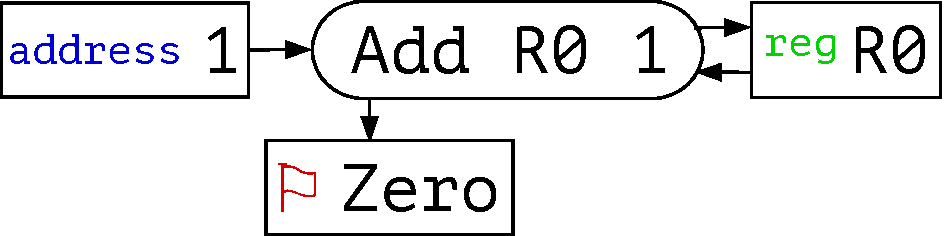
\includegraphics[width=7cm]{./fig/add.pdf}
  % \captionof{listing}{Another sub caption}
 \end{minipage}
 % \captionof{listing}{SomeCaption}
 %  \label{lst:representation_examples}
\end{figure}

The addition instruction semantics has only used the applicative combinators and thus
the same analysis capabilities could have been achieved with free applicative functors.
However, there are important instructions whose semantics cannot be implemented in terms
of the \hs{Applicative} interface, but still they do not require the heavy artillery of monads.

\subsubsection{\textbf{Example 2. Conditional jump}}

Selective functors allow to introduce limited dependencies between effectful computations.
It turns out, that they give just enough power to implement the semantics of conditional
jump instructions. A relative conditional jump offsets the program counter in case if a
certain condition, materialised in a microarchitectural flag, holds. For instance, some
instruction set might have a jump triggered by the fact that the result of the last addition
was zero:

\begin{minted}[xleftmargin=10pt]{haskell}
jumpZero :: Value -> ISA ()
jumpZero offset = let pc       = read PC
                      zeroSet  = (/=) <$> pure 0 <*> read (F Zero)
                      modifyPC = void $ write PC (fmap (+ offset) pc)
                  in whenS zeroSet modifyPC
\end{minted}

Here we use the aforementioned \hs{whenS} combinator to only execute the effect, i.e.
to modify the program counter, if the flag is set. By implementing this semantics in terms of
\hs{Selective} we achieve both the ability to implement an adequate simulator for the ISA and
to retain the possibilities for static analysis of programs by means of the \hs{getEffectsISA}
function:

\begin{figure}[!h]
 \begin{minipage}{0.45\textwidth}
\raggedleft
\begin{minted}[xleftmargin=10pt]{haskell}
@\ghci@ getEffectsISA (jumpZero 42)
[Read Zero,Read PC,Write PC]
\end{minted}
  % \captionof{listing}{Sub caption}
 \end{minipage}
 \begin{minipage}{0.45\textwidth}
  \centering
  
\includegraphics[width=7cm]{./fig/jumpZero.pdf}
  % \captionof{listing}{Another sub caption}
 \end{minipage}
 % \captionof{listing}{SomeCaption}
 %  \label{lst:representation_examples}
\end{figure}

Since the analysis is static, the resulting list of effects and data-flow graph are
over-approximated and show all effects that can possibly happen in the computation.
Note that it does not matter what argument we supply to \hs{jumpZero}, since it will
never get forced, e.g. the analysis will succeed and give us the same result even
if we supply \hs{undefined}.

\subsubsection{\textbf{Blocks of instructions}}

Once we have implemented the semantics for a desired subset of an ISA, we can construct the
semantics of sequences, or blocks, of instructions by simply composing the \hs{ISA} computations
using the applicative sequencing operator \hs{*>}:

\begin{minted}[xleftmargin=10pt]{haskell}
addAndJump :: ISA Value
addAndJump = add R0 1 *> jumpZero 42
\end{minted}

We can analyse the composed computations for its effects in the same way we analyse the
individual semantics:

\begin{figure}[!h]
 \begin{minipage}{0.45\textwidth}
\raggedleft
\begin{minted}[xleftmargin=10pt]{haskell}
@\ghci@ getEffectsISA addAndJump
[Read R0,Read 1,Write R0,Write Zero
,Read Zero,Read PC,Write PC]
\end{minted}
  % \captionof{listing}{Sub caption}
 \end{minipage}
 \begin{minipage}{0.45\textwidth}
  \centering
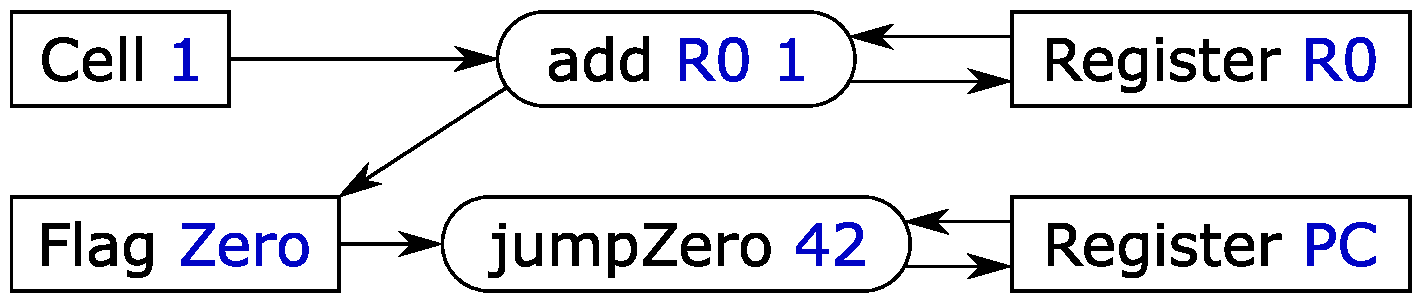
\includegraphics[width=7cm]{./fig/addAndJump.pdf}
  % \captionof{listing}{Another sub caption}
 \end{minipage}
 % \captionof{listing}{SomeCaption}
 %  \label{lst:representation_examples}
\end{figure}


Getting a flat list of effects that blocks of code perform is not very useful,
since they does not carry any explicit data-flow information. To mitigate this restriction,
we take the following approach. We create a (1) deeply-embedded assembly language and
(2) implement an interpreter which assigns a semantics to this language in terms of the
free selective construction. By doing this, we can then implement a mechanical procedure
which would construct \emph{data-flow graphs} of sequences of instructions, similar to
the ones shown in Fig.~\ref{fig-addAndJump-gcd} by overlaying the graphs for single instructions.
Note that if an instruction performs multiple read/writes of the same location, we will
deliberately merge them in the resulting graph.

\subsubsection{\textbf{Simulation}}

To implement a sequential simulator for the ISA, we need to follow the same path we did
when running the \hs{pingPongS} example in the \hs{IO} monad earlier in this section.
We need a natural transformation from the functor \hs{RW} to an appropriate target functor,
for example, an instance of \hs{MonadState ISAState}, where \hs{ISAState} is a product
type representing the state of the architecture, e.g. the registers, memory and flags.
For brevity, we present a simplified partial implementation of such a transformation which
only assigns interpretation to reading and writing registers:

\begin{minted}[xleftmargin=10pt]{haskell}
inState :: MonadState ISAState m => RW a -> m a
inState (Read k t) = t <$> case k of
    Reg r -> (Map.!) <$> (registers <$> get) <*> pure r
inState (Write k p t) = case k of
    Reg r -> do v <- runSelect inState p
                let regs' s = Map.insert r v (registers s)
                state (\s -> (t v, s {registers = regs' s}))
\end{minted}

To read a register, we simply lift the \hs{Data.Map} access combinator (the register bank
is represented as a mapping from register tags to data words). We need to apply the
continuation \hs{t :: Value -> a} to the result to make the types match. In order to write
an effectful value \hs{p} into a register, we need to evaluate it first; hence we call the
\hs{runSelect} function, which internally makes a recursive call to the \hs{inState} function
and thus acknowledges the effects of \hs{p}. We then adjust the register bank with the evaluated
value and construct a \hs{MonadState} computation with the \hs{state} function.

The \hs{inState} natural transformation gives interpretation to individual \hs{Read} and
\hs{Write} commands, and now this interpretation can be extended to any \hs{ISA}
computation by plugging it into a \hs{runSelect} call, which has already been once done in
the implementation of \hs{inState} itself.

\begin{minted}[xleftmargin=10pt]{haskell}
runProgram :: ISA a -> ISAState -> (a, ISAState)
runProgram f s = runState (runSelect inState f) s
\end{minted}

\subsubsection{\textbf{Restrictions}}

The free selective applicative construction in combination with the \hs{RW} functor
provide an abstraction expressive enough to express the
semantics of arithmetical, load and store instructions and conditional jumps. However,
they still lack the full expressive power of the monadic interface and are unable
to accommodate a very important instruction's semantics, namely the memory-indirect
load semantics. If we had a \hs{Monad} instance for \hs{ISA}, we could have written
the follow implementation:

\begin{minted}[xleftmargin=10pt]{haskell}
loadMI :: Register -> Address -> ISA Value
loadMI reg addr =
    read (Mem addr) >>= \x ->
    write (Reg reg) (read (Mem (toAddress x)))
\end{minted}

Here, we read from a memory cell and use the monadic bind operator to
peel of the \hs{ISA} type constructor of the value we read and use it in a consequent
memory read. However this semantics is, in principle, implementable using the
selective \hs{bindS} combinator, it is not feasible to do it this way since we would
not get any strong benefits. Specifically, since the \hs{getEffectsISA} function, which
performs static analysis of effects, constructs a conservative over-approximation, it
would always report something similar to this: \hs{[Read addr,Write reg, Write reg...},
which would contain as much instances of the \hs{Write} effects as much inhabitants there
are in the address datatype (usually a large power of two). Therefore, we lose static analysis.
Maybe we could get some benefit in simulation? No, unfortunately we, again, will not, since
\hs{bindS} cannot get magically translated to the monadic \hs{>>=}, but instead performs
explicit enumeration of inhabitants of the bound variable's type, which causes terrible performance regression comparing to a monadic implementation. Considering these arguments,
using \hs{bindS} for mimicking monadic behaviour is not feasible in our case and memory-indirect
load cannot be modelled in by means of the \hs{ISA} datatype.